\documentclass{article}
\usepackage{tikz, comment}
\usepackage{pifont}
\usepackage{fontspec}
\usetikzlibrary{arrows, decorations.markings, decorations.pathreplacing}
\begin{comment}
:Title: Not defined yet
:Slug: No name yet

Description Here.........
\end{comment}
\begin{document}\centering 

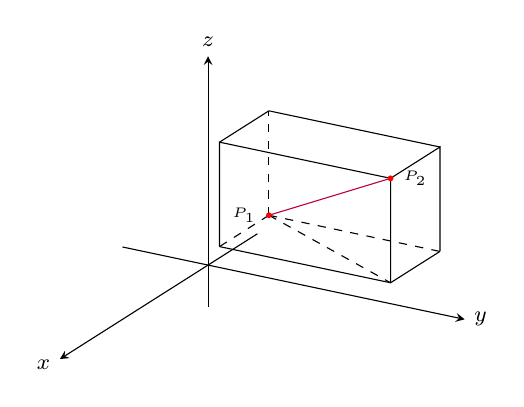
\begin{tikzpicture}[font=\footnotesize]
\pgfplotsset{compat=1.8}
\begin{axis}
[axis lines = center, view={120}{30}, ticks = none,
axis on top, xlabel = {$x$}, ylabel ={$y$}, zlabel ={$z$}, domain =0:1, y domain =0:1,
xmin =-2,
xmax =6,
ymin =-2,
ymax =6,
zmin =-2, 
zmax =10,
samples =10, samples y =40, z buffer =sort, 
every axis x label/.style={
    at={(ticklabel* cs:1)},
    anchor= east, yshift =-2
},
every axis y label/.style={
    at={(ticklabel* cs:1)},
    anchor= west,
},
every axis z label/.style={
    at={(ticklabel* cs:1)},
    anchor= south
},]

\addplot3[purple] coordinates
        {(1,2,4) (3,6,9)};

\addplot3[dashed] coordinates
        {(1,2,4) (3,2,4)};
\addplot3[dashed] coordinates
        {(1,2,4) (3,6,4)};
\addplot3[dashed] coordinates
        {(1,2,4) (1,2,9)};
\addplot3[dashed] coordinates    
        {(1,6,4) (1,2,4)};  
        
\addplot3[black] coordinates
        {(3,2,4) (3,6,4) (3,6,9)};
\addplot3[black] coordinates
        {(3,6,9) (3,2,9) (3,2,4)};  
\addplot3[black] coordinates
        {(1,2,9) (1,6,9)};
\addplot3[black] coordinates        
        {(1,2,9) (3,2,9)};        
\addplot3[black] coordinates        
        {(3,6,9) (1,6,9) (1,6,4)};
\addplot3[black] coordinates    
        {(1,6,4) (3,6,4)}; 

\node[label={180:{\tiny $P_1$}},circle,fill=red,inner sep=0.75pt] at (axis cs:1,2,4) {};
\node[label={0:{\tiny $P_2$}},circle,fill=red,inner sep=0.75pt] at (axis cs:3,6,9) {};
                                      
\end{axis}

\end{tikzpicture}
\end{document}